\section{Implementation}
The presented model is very simple yet shows a good accuracy on a wide band of frequencies. A possible improvement on the original discussion is the performance of its implementation, which is not public, but the authors mention \textit{`the computation time is about 5 minutes at a quad core
computer'}\cite{Hao-HsiangChuang2010ABCP} on a MATLAB script\autocite{5451081}.

This new implementation, titled \textbf{mem-pmod} (MEMory-PowerMODel) is \githublink{open source} and based mainly on C++ plus the support of Python to generate graphics, aims at a better performance and a higher degree of reusability.

\subsection{Features and Organization}
Mem-pmod is developed in C++ and is focused on the optimization of the process. It uses multithreading together with the highly optimized Eigen library to maximize performance. It offers:
\begin{itemize}
    \item Memory model fitting to experimental data as described from the paper
    \item Possibility to implement any generic fitting algorithm
    \item Model exporting and importing
\end{itemize}
It also includes some testing based on the GTest framework to check some of the available mechanisms.

\autoref{fig:program-flow} shows a typical flow of execution with the supported features.
\begin{figure}[htbp]
    \center
    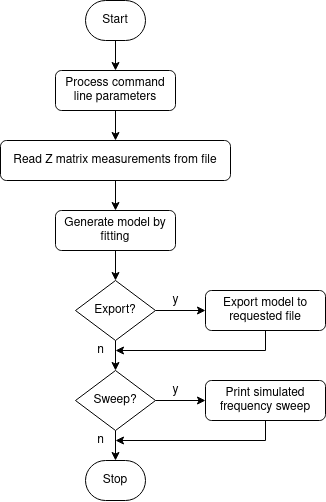
\includegraphics[width = 0.4\textwidth]{img/program-flowchart}
    \caption{Execution flow}
    \label{fig:program-flow}
\end{figure}
The program is organized in modules which may be grouped in three categories:
\begin{itemize}
    \item Models, which offer the infrastructure to build and interact with models
    \item Optimization, used by models to treat the fitting process as a generic optimization problem
    \item General control, which control the flow of the program and also offer some helpful, general purpose structures and functions
\end{itemize}

\subsection{Reading Measurements}
The measurements to be used as fitting data are stored in a text file and passed to the program as a command line parameter. Below is an example of a measurements file.
\begin{lstlisting}[backgroundcolor=\color{white},basicstyle=\tiny,breaklines=true]
f Z11 Z12 Z21 Z22
+1.000000e+06 (+1.253488e+01,-3.163626e+01) (-4.890959e+00,-2.934532e+01) (-4.890959e+00,-2.934532e+01) (+1.253488e+01,-3.163626e+01)
+1.047129e+06 (+1.251280e+01,-3.031854e+01) (-4.869922e+00,-2.792886e+01) (-4.869922e+00,-2.792886e+01) (+1.251280e+01,-3.031854e+01)
+1.096478e+06 (+1.248878e+01,-2.906428e+01) (-4.847045e+00,-2.657249e+01) (-4.847045e+00,-2.657249e+01) (+1.248878e+01,-2.906428e+01)
+1.148154e+06 (+1.246268e+01,-2.787069e+01) (-4.822186e+00,-2.527343e+01) (-4.822186e+00,-2.527343e+01) (+1.246268e+01,-2.787069e+01)
+1.202264e+06 (+1.243432e+01,-2.673511e+01) (-4.795195e+00,-2.402906e+01) (-4.795195e+00,-2.402906e+01) (+1.243432e+01,-2.673511e+01)
\end{lstlisting}
Each line contains, in order, the measurement frequency in Hz and the four elements of the $Z$ matrix in $\Omega$. Each element is a complex number, so it is represented as a pair (\textit{real part}, \textit{imaginary part}).

Measurements are stored in a specific structure:
\begin{lstlisting}[language=C++]
struct Measurements {
    std::vector<double> frequencies;
    std::vector<Matrix2> Z;
    unsigned port1;
    unsigned port2;
    std::size_t nsamples;
};
\end{lstlisting}
Which is initialized by
\begin{lstlisting}
Measurements readMeasurements(const std::string &fname, unsigned port1, unsigned port2);
\end{lstlisting}
The two ports from which the measurements were taken are specified as command line arguments.

\subsection{Geometric and Complete Models}
The overall memory is modeled in two steps: there is a model for a single TSection and the MemoryModel holds an array of TSections plus the PUL parameters. To keep the fitting process as clean as possible, models are also divided between Geometric and Complete. Geometric models only keep geometric information, Complete models expand the concept and also have additional information such as electrical parameters.

\begin{lstlisting}[title=Snippets for Geometric and Complete TSection]
class GeometricTSection {
public:
    GeometricTSection();
    ...
protected:
    double _length;
};

class TSection : private GeometricTSection {
public:
    TSection();
    ...
private:
    LumpedParameters _parameters;
};
\end{lstlisting}

\begin{lstlisting}[title=Snippets for Geometric and Complete MemoryModel]
template <std::size_t NPowerPorts>
class GeometricMemoryModel {
public:
    GeometricMemoryModel();
    ...
private:
    std::array<GeometricTSection, NPowerPorts> _sections;
};

template<std::size_t NPowerPorts>
class MemoryModel : private GeometricMemoryModel<NPowerPorts> {
public:
    MemoryModel();
    ...
private:
    std::array<TSection, NPowerPorts> _sections;
    PULParameters _pul_parameters;
};
\end{lstlisting}

\subsection{Fitting}
The MemoryModel class also offers the interface for fitting and this is where the multithreading action happens. This class offers a static method called \texttt{fit()} which sets up and passes the necessary information to the optimization module and finally initializes a MemoryModel based on the input data.
\begin{lstlisting}
static MemoryModel<NPowerPorts> fit(
        const Measurements &measurements,
        const std::array<double, NPowerPorts> lengths,
        pmod::optimization::Algorithm method = pmod::optimization::Algorithm::CDESCENT);
\end{lstlisting}
The function \texttt{fittingError()}, also offered from the same class, is the function that computes the error function described in \autoref{ssec:fitting}. Since this operation requires computing a Z matrix for each measured frequency, the measurements vector is divided in chunks which are computed in parallel through multithreading. The number of chunks depends on the hardware characteristics and is chosen to be as fast as possible. This is where the greatest improvement in performance happens.
\begin{lstlisting}
static double fittingError(
            const GeometricMemoryModel<NPowerPorts> &model,
            const PULParameters &pul_parameters,
            const Measurements &measurements,
            bool enable_threading = true);
\end{lstlisting}

The optimization module is the one that runs the actual optimization algorithm but treats everything as a generic multidimensional optimization problem. It offers the templated function
\begin{lstlisting}
template<std::size_t N>
Vector<N> optimize(Algorithm algorithm, std::function<double(Vector<N>)> function, Vector<N> x0, double threshold);
\end{lstlisting}
which automatically manages everything and allows for the choice of an optimization algorithm.

The original paper uses Powell's method whose manual implementation is difficult and outside the current scope of this project. The currently implemented algorithm is the Coordinate Descent algorithm, which can be slower and gets trapped in local minima more easily, but this should not be a problem at the moment.

\subsection{Importing and Exporting}
As mentioned above, it is also possible to import and export memory models. This is done by specific functions implemented for the MemoryModel and TSection classes which internally manage all the necessary steps. The current implementation simply dumps all the relevant parameters in order in a text file and then the importer just reads them.

\subsection{Results}
The results discussed in this section will be numerically different from the ones of the paper, but it is evident how the trend is perfectly matching. This is because:
\begin{enumerate}
    \item Measurements were manually generated since they are not available from the publication and they are not retrievable from the graphs because most functions overlap
    \item Section lengths were arbitrarily set since the paper only mentions the overall memory length ($\SI{4074}{\micro m}$) but does not mention the single section lengths nor the memory model or its layout where to retrieve them from
    \item The optimization algorithm is different
\end{enumerate}
In any case, everything was set up to be as reasonably close as possible to realistic inputs and the results from the paper.

\begin{figure}[htbp]
    \center
    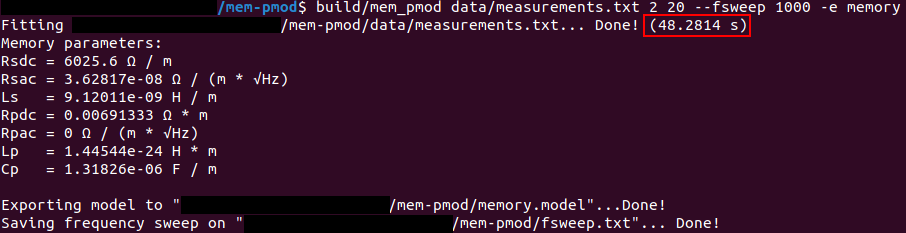
\includegraphics[width = 0.9\textwidth]{img/example_output}
    \caption{Example execution of mem-pmod}
    \label{fig:example-output}
\end{figure}
\autoref{fig:example-output} shows what a typical execution of mem-pmod looks like. The command line parameters specify, in order: the measurements file, the measurements ports, request a frequency sweep simulation with 10000 frequency samples (from 1 MHz to 10 GHz) and export the model to a file simply called \texttt{memory.model}.
\begin{table}[htbp]
    \center
    \begin{tabular}{|l|l|l|}
        \hline
        Quantity & Value \\ \hline
        Rsdc & $\SI{5312.13}{\Omega / m}$ \\ \hline
        Rsac & $\SI{0.0238141}{\Omega / (m * \sqrt{Hz})}$ \\ \hline
        Ls   & $\SI{9.18165e-09}{H / m}$ \\ \hline
        Rpdc & $\SI{0.00695145}{\Omega * m}$ \\ \hline
        Rpac & $\SI{1e-38}{\Omega / (m * \sqrt{Hz})}$ \\ \hline
        Lp   & $\SI{4.74466e-28}{H / m}$ \\ \hline
        Cp   & $\SI{1.31426e-06}{F / m}$ \\ \hline
    \end{tabular}
    \caption{Resulting PUL parameters from mem-pmod}
    \label{tab:pul-parameters}
\end{table}
The obtained PUL parameters visible in \autoref{fig:example-output} are also shown in \autoref{tab:pul-parameters} for clarity. Finally, the obtained frequency sweep is matched against the original measurements with the help of a Python script and the matplotlib library. The results of this comparison are shown in \autoref{fig:zmatrix}.

\begin{figure}[htbp]
    \center
    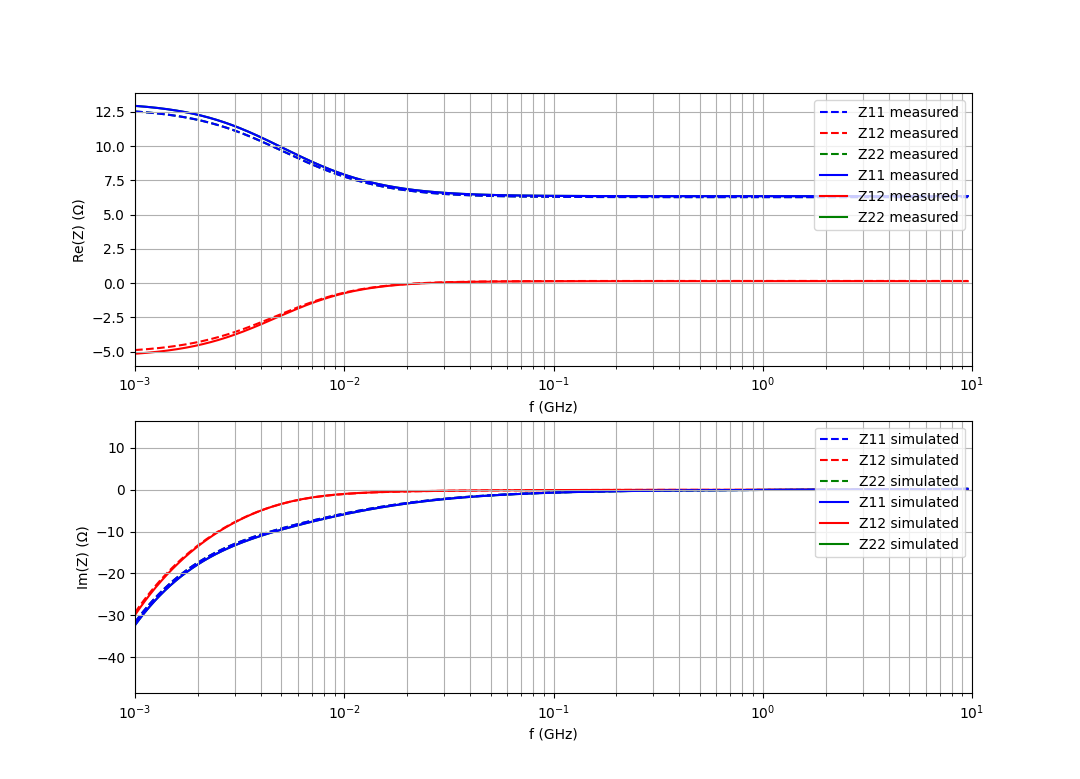
\includegraphics[width = 0.9\textwidth]{img/zmatrix}
    \caption{Results from mem-pmod against original measurements}
    \label{fig:zmatrix}
\end{figure}

\begin{figure}[htbp]
    \center
    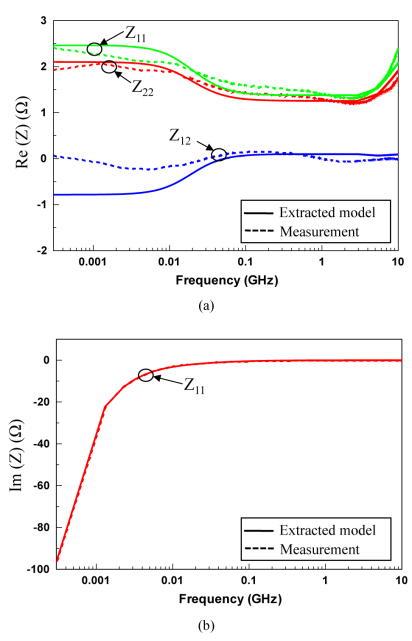
\includegraphics[width = 0.6\textwidth]{img/zmatrix-paper}
    \caption{Results from paper}
    \label{fig:zmatrix-paper}
\end{figure}


Comparing \autoref{fig:zmatrix} to \autoref{fig:zmatrix-paper}, the one generated from the researchers, shows how even though the numerical values differ the general behavior is the same.
